\documentclass[conference]{IEEEtran}
\IEEEoverridecommandlockouts
\usepackage[T1]{fontenc}
\usepackage[utf8]{inputenc}
\usepackage[brazilian]{babel}
\usepackage{cite}
\usepackage{amsmath,amssymb,amsfonts}
\usepackage{graphicx}
\usepackage{textcomp}
\usepackage{xcolor}
\usepackage{array}
\usepackage{booktabs}
\usepackage{multirow}
\usepackage{listings}
\usepackage{url}

\lstdefinestyle{vhdlstyle}{
    basicstyle=\ttfamily\scriptsize,
    breaklines=true,
    columns=fullflexible,
    frame=single,
    keepspaces=true,
    showstringspaces=false,
    tabsize=2
}
\lstset{style=vhdlstyle}

\begin{document}

\title{Implementação e Verificação de Processador MIPS Simplificado com FSM em VHDL\\
{\footnotesize Relatório de Laboratório -- Trabalho 2}}

\author{\IEEEauthorblockN{Discente: Erick Gleisson Batista Sebba}
\IEEEauthorblockA{\textit{Laboratório de Arquitetura de Computadores}\\
\textit{Universidade Federal de Mato Grosso -- FAENG}\\
Engenharia de Computação -- Turma VE2}}

\maketitle

\begin{abstract}
Este relatório apresenta a implementação e a verificação comportamental de um processador MIPS simplificado para instruções do tipo R. O projeto integra uma ROM de operandos, uma RAM de resultados, uma ULA de 32 bits e uma unidade de controle baseada em máquina de estados finitos. A verificação foi conduzida por testbench modular, com geração automática de estímulos, monitoramento dos resultados e comparação com cálculos manuais para operações ADD, SUB, ADDU e SUBU. Os resultados obtidos no console de simulação e nos diagramas de tempo confirmam a sequência correta de leitura dos operandos, execução aritmética e escrita na RAM.
\end{abstract}

\begin{IEEEkeywords}
MIPS, VHDL, ULA, FSM, testbench modular, Riviera-PRO, EDA Playground, complemento de dois, overflow.
\end{IEEEkeywords}

\section{Introdução}
O objetivo do laboratório foi implementar uma arquitetura simplificada inspirada no conjunto de instruções MIPS, restrita a instruções aritméticas do tipo R. O sistema desenvolvido recebe uma instrução de 32 bits, decodifica os campos \textit{rs}, \textit{rt}, \textit{rd} e \textit{funct}, busca os operandos em uma ROM, executa a operação na ULA e grava o resultado na RAM. A coordenação do fluxo de dados é feita por uma unidade de controle implementada como máquina de estados finitos (FSM).

A atividade também exigiu uma metodologia de verificação que não dependesse apenas da inspeção visual das formas de onda. Por isso, foi construído um testbench modular com geração de estímulos e checagem automática, emitindo mensagens de validação no console do simulador. O ambiente utilizado foi o EDA Playground com Aldec Riviera-PRO 2025.04 e padrão VHDL-2019.

\section{Documentação da Arquitetura}

\subsection{Formato da Instrução MIPS Tipo R}
As instruções do tipo R possuem 32 bits e utilizam o campo \textit{funct} para selecionar a operação aritmética. O campo \textit{op} permanece em zero, pois a operação é definida pelo código de função. A Tabela~\ref{tab:rtype} mostra o mapeamento utilizado.

\begin{table}[!t]
\caption{Formato da instrução MIPS tipo R utilizado no projeto}
\label{tab:rtype}
\centering
\begin{tabular}{c c c c c c c}
\toprule
Campo & op & rs & rt & rd & shamt & funct \\
\midrule
Bits & 31--26 & 25--21 & 20--16 & 15--11 & 10--6 & 5--0 \\
Uso & 000000 & ROM A & ROM B & RAM & 00000 & ULA \\
\bottomrule
\end{tabular}
\end{table}

No projeto, \textit{rs} endereça o primeiro operando na ROM, \textit{rt} endereça o segundo operando, \textit{rd} indica o endereço de escrita na RAM e \textit{funct} é enviado diretamente à ULA. Foram consideradas as funções ADD, ADDU, SUB e SUBU, conforme a Tabela~\ref{tab:funct}.

\begin{table}[!t]
\caption{Códigos de função implementados na ULA}
\label{tab:funct}
\centering
\begin{tabular}{c c c}
\toprule
Operação & Decimal & Funct binário \\
\midrule
ADD  & 32 & 100000 \\
ADDU & 33 & 100001 \\
SUB  & 34 & 100010 \\
SUBU & 35 & 100011 \\
\bottomrule
\end{tabular}
\end{table}

\subsection{Organização Estrutural}
A arquitetura top level, denominada \texttt{processador\_top}, interliga quatro blocos principais: ROM, RAM, ULA e unidade de controle. A ROM \texttt{rom\_32x32} armazena 32 palavras de 32 bits e fornece os operandos. A RAM \texttt{ram\_32x32} armazena os resultados. A ULA \texttt{ula} executa operações aritméticas combinacionais. A unidade \texttt{control\_unit} gera os endereços e sinais de controle a partir da instrução e do protocolo \texttt{start}/\texttt{done}.

A Figura~\ref{fig:arch} resume as conexões estruturais implementadas. O barramento \texttt{rom\_data\_s} fornece o operando B diretamente para a ULA, enquanto o operando A é preservado em \texttt{reg\_a\_internal} após a leitura do endereço \textit{rs}. O resultado da ULA é conectado ao barramento de entrada da RAM.

\begin{figure}[!t]
\centering
\fbox{\begin{minipage}{0.92\linewidth}
\centering
\texttt{instruction[31:0]} $\rightarrow$ \texttt{control\_unit}\\[2pt]
\texttt{rs/rt} $\rightarrow$ \texttt{rom\_addr} $\rightarrow$ \texttt{ROM} $\rightarrow$ \texttt{rom\_data}\\[2pt]
\texttt{ROM[rs]} $\rightarrow$ \texttt{reg\_a\_internal} $\rightarrow$ \texttt{ULA.a}\\[2pt]
\texttt{ROM[rt]} $\rightarrow$ \texttt{ULA.b}; \quad \texttt{funct} $\rightarrow$ \texttt{ULA}\\[2pt]
\texttt{ULA.result} $\rightarrow$ \texttt{RAM.di}; \quad \texttt{rd} $\rightarrow$ \texttt{RAM.addr}
\end{minipage}}
\caption{Diagrama estrutural simplificado do processador implementado.}
\label{fig:arch}
\end{figure}

\subsection{Máquina de Estados Finitos}
A unidade de controle foi implementada com o tipo de estado obrigatório \texttt{state\_type is (IDLE, FETCH\_A, FETCH\_B, STORE\_RAM, FINISHED)}. A Figura~\ref{fig:fsm} mostra o diagrama de transição da FSM.

\begin{figure}[!t]
\centering
\fbox{\begin{minipage}{0.92\linewidth}
\centering
\texttt{IDLE} $\xrightarrow{start='1'}$ \texttt{FETCH\_A} $\rightarrow$ \texttt{FETCH\_B} $\rightarrow$ \texttt{STORE\_RAM} $\rightarrow$ \texttt{FINISHED}\\[4pt]
\texttt{FINISHED} $\xrightarrow{start='0'}$ \texttt{IDLE}
\end{minipage}}
\caption{Diagrama de transição de estados da unidade de controle.}
\label{fig:fsm}
\end{figure}

A Tabela~\ref{tab:control} detalha os sinais de controle gerados em cada estado. No estado \texttt{FETCH\_A}, a ROM recebe o endereço \textit{rs} e o dado é capturado internamente. No estado \texttt{FETCH\_B}, a ROM passa a receber \textit{rt}, permitindo que a ULA opere com A armazenado e B vindo da ROM. Em \texttt{STORE\_RAM}, \texttt{ram\_we} é ativado para gravar o resultado no endereço \textit{rd}. Por fim, \texttt{FINISHED} sinaliza \texttt{done}.

\begin{table}[!t]
\caption{Sinais de controle por estado da FSM}
\label{tab:control}
\centering
\scriptsize
\setlength{\tabcolsep}{2.5pt}
\begin{tabular}{c c c c c c}
\toprule
Estado & \texttt{rom\_addr} & \texttt{ram\_addr} & \texttt{ram\_we} & \texttt{reg\_a} & \texttt{done} \\
\midrule
IDLE & 0 & 0 & 0 & mantém & 0 \\
FETCH\_A & rs & 0 & 0 & captura & 0 \\
FETCH\_B & rt & 0 & 0 & mantém & 0 \\
STORE\_RAM & 0 & rd & 1 & mantém & 0 \\
FINISHED & 0 & 0 & 0 & mantém & 1 \\
\bottomrule
\end{tabular}
\end{table}

\section{Implementação e Síntese}

\subsection{Geração da ROM}
A ROM foi gerada a partir de um script Python com 32 posições de 32 bits e valores inteiros entre 0 e 200. Para manter a simulação reprodutível, foram utilizados os valores fixos mostrados na Tabela~\ref{tab:rom}.

\begin{table}[!t]
\caption{Conteúdo da ROM usado na simulação}
\label{tab:rom}
\centering
\scriptsize
\begin{tabular}{c c c c c c c c}
\toprule
0 & 1 & 2 & 3 & 4 & 5 & 6 & 7 \\
5 & 6 & 123 & 79 & 50 & 30 & 100 & 25 \\
\midrule
8 & 9 & 10 & 11 & 12 & 13 & 14 & 15 \\
60 & 85 & 40 & 15 & 119 & 65 & 90 & 10 \\
\midrule
16 & 17 & 18 & 19 & 20 & 21 & 22 & 23 \\
150 & 45 & 105 & 20 & 70 & 200 & 55 & 130 \\
\midrule
24 & 25 & 26 & 27 & 28 & 29 & 30 & 31 \\
27 & 89 & 110 & 35 & 145 & 12 & 180 & 120 \\
\bottomrule
\end{tabular}
\end{table}

\subsection{Módulos VHDL}
A implementação foi dividida em cinco módulos. A ROM é combinacional e acessa o vetor constante pelo índice \texttt{to\_integer(unsigned(addr))}. A RAM possui escrita síncrona, habilitada por \texttt{we} na borda de subida do clock, e leitura assíncrona. A ULA é combinacional e utiliza \texttt{signed}, \texttt{unsigned} e \texttt{resize} da biblioteca \texttt{numeric\_std} para realizar operações em 33 bits. Nas operações sinalizadas, o \textit{overflow} é indicado quando o bit 32 difere do bit 31 do resultado estendido. Nas operações sem sinal, ADDU utiliza o carry de 33 bits e SUBU mantém \texttt{ovfl='0'}.

A unidade de controle foi escrita com um processo sequencial para transições de estado e captura de \texttt{reg\_a\_internal}, além de um processo combinacional para geração das saídas. O top level instancia \texttt{U\_ROM}, \texttt{U\_RAM}, \texttt{U\_ULA} e \texttt{U\_FSM}, conectando \texttt{ram\_di\_s <= ula\_result\_s}, \texttt{ula\_b\_s <= rom\_data\_s} e \texttt{funct\_s <= instruction(5 downto 0)}. A captura RTL obtida confirma visualmente essa interligação estrutural entre os blocos.

\subsection{Síntese e Recursos de Hardware}
A implementação foi desenvolvida e verificada no EDA Playground, utilizando o simulador Aldec Riviera-PRO 2025.04. Além da simulação comportamental, foi obtida a captura RTL da arquitetura do projeto, apresentada na Figura~\ref{fig:rtl}. Essa figura evidencia a interconexão estrutural entre ROM, unidade de controle, ULA e RAM. O ambiente utilizado, entretanto, não gera o \textit{Compilation Report} físico do Intel Quartus com ALUTs e registradores. Assim, a Tabela~\ref{tab:resources} explicita o que foi validado e quais itens dependeriam de uma síntese posterior no Quartus.

\begin{figure*}[!t]
\centering
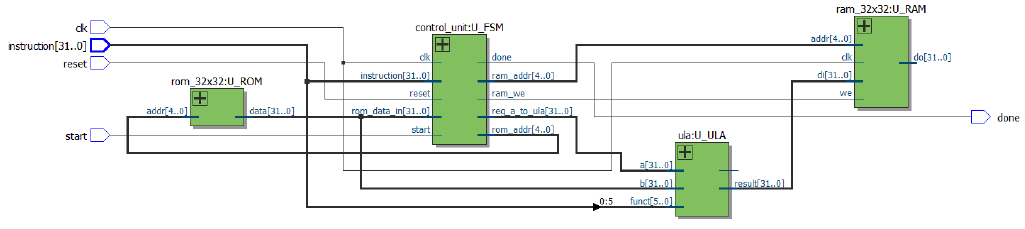
\includegraphics[width=0.98\textwidth]{arquitetura_do_trabalho.png}
\caption{Captura RTL da arquitetura do projeto, mostrando a interligação entre \texttt{U\_ROM}, \texttt{U\_FSM}, \texttt{U\_ULA} e \texttt{U\_RAM}.}
\label{fig:rtl}
\end{figure*}

\begin{table}[!t]
\caption{Resumo de síntese e recursos no ambiente utilizado}
\label{tab:resources}
\centering
\scriptsize
\setlength{\tabcolsep}{3pt}
\begin{tabular}{p{0.35\linewidth} p{0.55\linewidth}}
\toprule
Item & Situação \\
\midrule
Ambiente usado & EDA Playground com Aldec Riviera-PRO 2025.04 \\
Compilação VHDL & 0 erros e 0 avisos no conjunto principal \\
RTL/arquitetura & Captura incluída na Figura~\ref{fig:rtl} \\
Logic Elements/ALUTs & Não gerado; requer síntese no Intel Quartus \\
Registradores físicos & Não gerado; requer \textit{Compilation Report} do Quartus \\
Evidência funcional & Waveforms e \textit{Assertion Report} confirmam as operações \\
\bottomrule
\end{tabular}
\end{table}

\section{Verificação Modular e Automatizada}

\subsection{Estratégia de Verificação}
O testbench foi organizado em duas responsabilidades. A parte de \textit{Stimulus} gera clock, reset, instruções de 32 bits e pulsos de \texttt{start}. A parte de \textit{Checker} aguarda \texttt{done='1'} e emite mensagens \texttt{report} indicando o resultado esperado e o endereço de RAM escrito. A montagem da instrução foi encapsulada na função \texttt{make\_rtype}, e a procedure \texttt{run\_op} executa cada cenário de teste.

Foram verificados cinco cenários: ADD, SUB, ADDU, SUBU e uma subtração com resultado negativo em complemento de dois. A Tabela~\ref{tab:manual} apresenta a validação manual usada como referência.

\begin{table*}[!t]
\caption{Validação manual das operações simuladas}
\label{tab:manual}
\centering
\begin{tabular}{c c c c c c c c}
\toprule
Instrução & rs & A=ROM[rs] & rt & B=ROM[rt] & rd & Resultado esperado & Hex 32 bits \\
\midrule
ADD & 0 & 5 & 1 & 6 & 2 & $+11$ & 0x0000000B \\
SUB & 3 & 79 & 4 & 50 & 5 & $+29$ & 0x0000001D \\
ADDU & 6 & 100 & 7 & 25 & 8 & $+125$ & 0x0000007D \\
SUBU & 9 & 85 & 10 & 40 & 11 & $+45$ & 0x0000002D \\
SUB\_NEG & 5 & 30 & 2 & 123 & 12 & $-93$ & 0xFFFFFFA3 \\
\bottomrule
\end{tabular}
\end{table*}

No caso \texttt{SUB\_NEG}, o cálculo manual é $30-123=-93$. Em complemento de dois de 32 bits, esse valor corresponde a \texttt{0xFFFFFFA3}, observado no barramento \texttt{ram\_di\_s} durante o pulso de escrita.

\subsection{Script TCL}
O script de simulação inicializa a biblioteca de trabalho, compila os módulos, instancia o testbench, organiza sinais no visualizador de ondas, gera VCD e executa a simulação por 1000 ns. O trecho principal é mostrado no Código~\ref{lst:tcl}.

\begin{lstlisting}[caption={Script TCL utilizado na simulação},label={lst:tcl}]
vlib work
vcom -2019 -dbg rom_32x32.vhd ram_32x32.vhd ula.vhd control_unit.vhd design.vhd testbench.vhd
vsim +access+r work.tb_top
add wave /tb_top/clk
add wave /tb_top/reset
add wave /tb_top/start
add wave /tb_top/done
add wave -hex /tb_top/instruction
add wave /tb_top/DUT/U_FSM/state
add wave -uns /tb_top/DUT/rom_addr_s
add wave -uns /tb_top/DUT/rom_data_s
add wave -uns /tb_top/DUT/ula_a_s
add wave -uns /tb_top/DUT/ula_result_s
add wave /tb_top/DUT/ula_ovfl_s
add wave -uns /tb_top/DUT/ram_addr_s
add wave /tb_top/DUT/ram_we_s
add wave -uns /tb_top/DUT/ram_di_s
vcd file dump.vcd
vcd add -r /tb_top/*
run 1000ns
exit
\end{lstlisting}

\section{Diagramas de Tempo}
As Figuras~\ref{fig:wave1} e~\ref{fig:wave2} mostram as formas de onda obtidas no EPWave. Os sinais confirmam que cada instrução percorre a sequência \texttt{IDLE -> FETCH\_A -> FETCH\_B -> STORE\_RAM -> FINISHED}. O endereço da ROM aponta primeiro para \textit{rs} e depois para \textit{rt}; o registrador interno mantém o operando A; a ULA apresenta o resultado no barramento; e \texttt{ram\_we\_s} fica ativo apenas no estado de escrita.

\begin{figure}[!t]
\centering
\includegraphics[width=\linewidth]{image1_lab2_flat.png}
\caption{Forma de onda com sinais de dados da ROM, ULA e RAM.}
\label{fig:wave1}
\end{figure}

\begin{figure*}[!t]
\centering
\includegraphics[width=0.95\textwidth]{image2_lab2_flat.png}
\caption{Forma de onda completa com sinais internos do top level e da unidade de controle.}
\label{fig:wave2}
\end{figure*}

Durante as operações, \texttt{ram\_addr\_s} assume os endereços de destino 2, 5, 8, 11 e 12, enquanto \texttt{ram\_di\_s} apresenta, respectivamente, \texttt{0x0000000B}, \texttt{0x0000001D}, \texttt{0x0000007D}, \texttt{0x0000002D} e \texttt{0xFFFFFFA3}. O sinal \texttt{done} sobe após a escrita na RAM, indicando a conclusão da instrução. O aviso de \textit{metavalue} no tempo 0 ps ocorre antes da estabilização inicial dos endereços e não afeta a validação.

\section{Relatório de Verificação}
O Código~\ref{lst:log} transcreve o log de simulação. A compilação do conjunto principal foi concluída com 0 erros e 0 avisos, e o checker confirmou os resultados esperados para todas as operações testadas.

\begin{lstlisting}[caption={Log de verificação emitido pelo simulador},label={lst:log}]
# ACOM: Compile success 0 Errors 0 Warnings  Analysis time : 40.0 [ms]
# EXECUTION:: NOTE   : [CHECKER] ADD     : ROM[0]=5 op ROM[1]=6 => esperado=11 gravado em RAM[2]
# EXECUTION:: Time: 75 ns,  Iteration: 0,  Instance: /tb_top,  Process: line__60.
# EXECUTION:: NOTE   : [CHECKER] SUB     : ROM[3]=79 op ROM[4]=50 => esperado=29 gravado em RAM[5]
# EXECUTION:: Time: 175 ns,  Iteration: 0,  Instance: /tb_top,  Process: line__60.
# EXECUTION:: NOTE   : [CHECKER] ADDU    : ROM[6]=100 op ROM[7]=25 => esperado=125 gravado em RAM[8]
# EXECUTION:: Time: 275 ns,  Iteration: 0,  Instance: /tb_top,  Process: line__60.
# EXECUTION:: NOTE   : [CHECKER] SUBU    : ROM[9]=85 op ROM[10]=40 => esperado=45 gravado em RAM[11]
# EXECUTION:: Time: 375 ns,  Iteration: 0,  Instance: /tb_top,  Process: line__60.
# EXECUTION:: NOTE   : [CHECKER] SUB_NEG : ROM[5]=30 op ROM[2]=123 => esperado=-93 gravado em RAM[12]
# EXECUTION:: Time: 475 ns,  Iteration: 0,  Instance: /tb_top,  Process: line__60.
# EXECUTION:: NOTE   : === SIMULACAO CONCLUIDA ===
# EXECUTION:: Time: 525 ns,  Iteration: 0,  Instance: /tb_top,  Process: line__60.
\end{lstlisting}



\section{Trechos Essenciais de Implementação}
Como a Figura~\ref{fig:rtl} já mostra a arquitetura estrutural, esta seção resume apenas os trechos de VHDL necessários para relacionar o diagrama com o funcionamento do processador. O objetivo é evidenciar o caminho de dados, a decodificação da instrução e a automação da verificação.

\subsection{Caminho de Dados no Top Level}
No \texttt{processador\_top}, o campo \texttt{funct} é enviado à ULA, o dado atual da ROM alimenta o operando B e o resultado da ULA é conectado à entrada da RAM. A FSM controla os endereços e o pulso de escrita.

\begin{lstlisting}[caption={Conexões principais entre ROM, ULA, RAM e FSM},label={lst:topconnect}]
funct_s  <= instruction(5 downto 0);
ula_b_s  <= rom_data_s;
ram_di_s <= ula_result_s;

U_ROM : entity work.rom_32x32
  port map(addr => rom_addr_s, data => rom_data_s);
U_RAM : entity work.ram_32x32
  port map(clk => clk, we => ram_we_s, addr => ram_addr_s,
           di => ram_di_s, do => ram_do_s);
U_ULA : entity work.ula
  port map(a => ula_a_s, b => ula_b_s, funct => funct_s,
           result => ula_result_s, ovfl => ula_ovfl_s);
U_FSM : entity work.control_unit
  port map(clk => clk, reset => reset, start => start,
           instruction => instruction, rom_data_in => rom_data_s,
           rom_addr => rom_addr_s, ram_addr => ram_addr_s,
           ram_we => ram_we_s, reg_a_to_ula => ula_a_s,
           done => done);
\end{lstlisting}

Esse trecho demonstra o caminho de dados principal: a FSM escolhe o endereço da ROM, a ROM entrega o operando, a ULA executa a operação e a RAM grava o resultado quando \texttt{ram\_we\_s='1'}.

\subsection{Decodificação da Instrução e FSM}
A unidade de controle decodifica os campos MIPS tipo R por fatiamento direto da instrução. Em seguida, a FSM define qual endereço será enviado à ROM ou à RAM em cada etapa do processamento.

\begin{lstlisting}[caption={Decodificação dos campos e ações por estado},label={lst:fsmconnect}]
rs_addr <= instruction(25 downto 21);
rt_addr <= instruction(20 downto 16);
rd_addr <= instruction(15 downto 11);

case state is
  when FETCH_A   => rom_addr <= rs_addr;
  when FETCH_B   => rom_addr <= rt_addr;
  when STORE_RAM => ram_addr <= rd_addr; ram_we <= '1';
  when FINISHED  => done <= '1';
  when others    => null;
end case;
\end{lstlisting}

O primeiro operando precisa ser preservado antes da leitura do segundo. Por isso, ao sair de \texttt{FETCH\_A}, o dado atual da ROM é armazenado em \texttt{reg\_a\_internal}; no ciclo seguinte, a ROM passa a apontar para \textit{rt}, mas o valor de A permanece disponível para a ULA.

\begin{lstlisting}[caption={Captura do operando A antes da leitura de B}]
when FETCH_A =>
  reg_a_internal <= rom_data_in;
  state <= FETCH_B;
\end{lstlisting}

\subsection{Operação da ULA}
A ULA recebe dois operandos de 32 bits e o campo \texttt{funct}. Para ADD e SUB sinalizados, os operandos são convertidos para \texttt{signed} com 33 bits, permitindo verificar overflow pela comparação entre os bits 32 e 31 do resultado estendido. Para ADDU e SUBU, a operação é tratada como não sinalizada.

\begin{lstlisting}[caption={Seleção da operação aritmética pelo campo funct},label={lst:ulasnippet}]
sa := resize(signed(a), 33);
sb := resize(signed(b), 33);
ua := resize(unsigned(a), 33);
ub := resize(unsigned(b), 33);

case funct is
  when "100000" => rs := sa + sb;  -- ADD
  when "100001" => ru := ua + ub;  -- ADDU
  when "100010" => rs := sa - sb;  -- SUB
  when "100011" => ru := ua - ub;  -- SUBU
  when others   => result <= (others => '0');
end case;
\end{lstlisting}

\subsection{Acesso às Memórias}
A ROM é lida de forma combinacional: ao receber \texttt{rom\_addr\_s}, ela entrega imediatamente a palavra correspondente em \texttt{rom\_data\_s}. A RAM grava apenas no estado \texttt{STORE\_RAM}, pois esse é o único estado em que a FSM ativa \texttt{ram\_we\_s}.

\begin{lstlisting}[caption={Leitura da ROM e escrita síncrona da RAM}]
-- ROM: leitura combinacional
rom_data <= ROM(to_integer(unsigned(rom_addr)));

-- RAM: escrita somente quando ram_we_s = '1'
if rising_edge(clk) then
  if ram_we_s = '1' then
    RAM(to_integer(unsigned(ram_addr_s))) <= ram_di_s;
  end if;
end if;
\end{lstlisting}

Assim, o fluxo temporal observado nos waveforms é coerente com a FSM: primeiro \textit{rs} seleciona A, depois \textit{rt} seleciona B, e finalmente \textit{rd} seleciona o endereço de destino da RAM.

\subsection{Testbench Modular e Checker}
O testbench automatiza a validação por meio da procedure \texttt{run\_op}. Ela monta uma instrução tipo R, ativa \texttt{start}, espera \texttt{done} e emite um \texttt{report} com o valor esperado calculado a partir da ROM conhecida.

\begin{lstlisting}[caption={Trecho do checker automatizado no testbench},label={lst:checkersnippet}]
instruction <= make_rtype(rs_i, rt_i, rd_i, funct_i);
start <= '1';
wait until done = '1';

report "[CHECKER] " & op_str &
       ": ROM[" & integer'image(rs_i) & "]=" &
       integer'image(ROM_VAL(rs_i)) &
       " op ROM[" & integer'image(rt_i) & "]=" &
       integer'image(ROM_VAL(rt_i)) &
       " => esperado=" & integer'image(expected) &
       " gravado em RAM[" & integer'image(rd_i) & "]"
       severity note;

start <= '0';
\end{lstlisting}

Essa separação deixa claro o papel do \textit{Stimulus}, que aplica entradas ao DUT, e do \textit{Checker}, que calcula e registra a saída esperada para cada instrução.

\subsection{Script Python da ROM}
O script Python usado no Google Colab/ambiente auxiliar gera os valores aleatórios e escreve a constante VHDL da ROM. Para a simulação documentada, os valores foram fixados conforme a Tabela~\ref{tab:rom}, permitindo conferir manualmente os resultados.

\begin{lstlisting}[caption={Núcleo do gerador Python da ROM}]
values = [random.randint(0, 200) for _ in range(32)]
entries = []
for i, val in enumerate(values):
    entries.append(f' {i} => x"{val:08X}"')

vhdl_content += ",\n".join(entries)
vhdl_content += "\n);\nbegin\n"
vhdl_content += "  data <= ROM(to_integer(unsigned(addr)));\n"
\end{lstlisting}

\section{Conclusão}
O processador MIPS simplificado foi implementado conforme a arquitetura proposta no laboratório. A FSM executou corretamente a sequência de busca do operando A, busca do operando B, escrita do resultado na RAM e sinalização de término. A ULA produziu os resultados esperados para operações sinalizadas e não sinalizadas, incluindo a subtração com resultado negativo representado em complemento de dois. A validação por testbench modular e \texttt{report} confirmou automaticamente os resultados, enquanto os waveforms evidenciaram os sinais internos exigidos pelo enunciado.

A captura RTL acrescentada evidencia a arquitetura estrutural do projeto e confirma as conexões entre os módulos principais. Como o trabalho foi desenvolvido no EDA Playground, ainda não houve geração de relatório físico de ALUTs e registradores do Quartus; essa parte dependeria de uma síntese FPGA completa. Mesmo assim, a documentação dos trechos de interconexão, a descrição das ações da FSM, os waveforms e o relatório automático do checker confirmaram o funcionamento lógico da arquitetura.

\begin{thebibliography}{00}
\bibitem{patterson} D. A. Patterson and J. L. Hennessy, \textit{Computer Organization and Design: The Hardware/Software Interface}, 5th ed. Morgan Kaufmann, 2014.
\bibitem{pedroni} V. A. Pedroni, \textit{Circuit Design and Simulation with VHDL}. MIT Press, 2010.
\bibitem{ieee1076} IEEE, \textit{IEEE Standard VHDL Language Reference Manual}, IEEE Std 1076-2008, 2009.
\bibitem{aldec} Aldec, \textit{Riviera-PRO User Documentation}, Aldec Inc.
\end{thebibliography}

\end{document}
